% This is LLNCS.DEM the demonstration file of
% the LaTeX macro package from Springer-Verlag
% for Lecture Notes in Computer Science,
% version 2.3 for LaTeX2e
%
\documentclass{llncs}
%
\usepackage{makeidx}  % allows for indexgeneration
\usepackage{graphicx}
\usepackage{amssymb}
\usepackage{listings}
\usepackage{tabularx}
\usepackage{booktabs}
\usepackage{subscript}
\usepackage{amsmath}
\lstset{breaklines=true, basicstyle=\scriptsize\ttfamily}

%
\begin{document}
%
\frontmatter          % for the preliminaries
%
\pagestyle{headings}  % switches on printing of running heads
%\addtocmark{Hamiltonian Mechanics} % additional mark in the TOC
%
%
\mainmatter              % start of the contributions
%
\title{Exploiting Semantic Web Datasets: a Summarization Based Approach}

%
\titlerunning{Exploiting Semantic Web Datasets: a Summarization Based Approach}  % abbreviated title (for running head)
%                                     also used for the TOC unless
%                                     \toctitle is used
%
\author{Honghan Wu\inst{1} \and Boris Villazon-Terrazas\inst{2} \and Jeff Z. Pan\inst{1} \and Jose Manuel Gomez-Perez\inst{2}}
%
\authorrunning{Wu et al.}   % abbreviated author list (for running head)
%
%%%% list of authors for the TOC (use if author list has to be modified)
%\tocauthor{Panos Alexopoulos, Manolis Wallace}
%
\institute{Department of
Computing Science, University of Aberdeen, UK, \\ \email{\{honghan.wu,jeff.z.pan\}@abdn.ac.uk} \and
iSOCO, Intelligent Software Components S.A., Spain,\\
\email{bvillazon,jmgomez@isoco.com} }


\maketitle              % typeset the title of the contribution

%**************************************************************
%**************************************************************
%**************************************************************


\begin{abstract}
In the last years, we have witnessed vast increase of Linked Data datasets not only in the volume, but also in number of various domains and across different sectors. However, due to the nature and techniques used within Linked Data, it is non-trivial work for normal users to quickly understand what is within the datasets, and even for tech-users to efficiently exploit the datasets. In this paper, we propose a summarisation based approach to guide the exploitation of Linked Data. 
\end{abstract}

\section{Introduction}\label{sec:Introduction}
Lately there is an increasing variety of Linked Data datasets coming from different data sources. However, these datasets are of varying quality ranging from extensively curated datasets to crowd-sourced or extracted data to often relatively low quality. This lack of data quality poses problems to developers aiming to seamlessly consume and integrate Linked Data in their applications.

There are some 
In \cite{} authors group the linked data quality features into six main dimensions (1) conextual dimensions, (2) trust dimensions, (3) intrinsic dimensions, (4) accessibility dimensions, (5) accessibility dimensions, (6) representational dimensions, and (7) dataset dynamicity


Verifiability.- Verifiability refers to the degree by which a data consumer can access the correctness of a dataset and as consequence its trustworthiness


however, data in the LOD cloud has not been necessarily curated, and tools are required to detect possible ambiguities and quality problems ... 

Linked Data has a number of challenges 



There are many research works that try to define a set of key points for data quality \cite{}. 


One important aspect of the Linked Data community is to measure the quality of a datasets. In spite \emph{quality} is a subjective factor, we can list some key points regarding the quality of the dataset \cite{}, namely

\begin{itemize}
	\item Accuracy - are facts actually correct?
	\item Intelligibility - are there human readable labels on things?
	\item Referential correspondence - are resources identified consistently without duplication?
	\item Completeness - do you have all the data you expect?
	\item Boundedness - do you have just the data you expect or is it polluted with irrelevant data?
	\item Typing - are nodes properly typed as resources or just string literals?
	\item Modeling correctness - is the logical structure of the data correct?
	\item Modeling granularity - does the modeling capture enough information to be useful?
	\item Connectedness - do combined datasets join at the right points?
	\item Isomorphism - are combined datasets modeled in a compatible way?
	\item Currency - is it up to date?
	\item Directionality - is it consistent in the direction of relations?
	\item Attribution - can you tell where portions of the data came from?
	\item History - can you tell who edited the data and when?
	\item Internal consistency - does the data contradict itself?
	\item Licensed - is the license for use clear?
	\item Sustainable - is there a credible basis for believing the data will be maintained?
	\item Authoritative- is the provider of the data a credible authority on the subject?
\end{itemize}

Linked Data quality measures might include:
\begin{itemize}
	\item incoming and outgoing links
	\item used vocabularies, and properties
	\item adherence to property range restrictions, their values, etc.
\end{itemize}

However, the first step to get qualiaty of the data is get the snapshot, a summary, of the linked data dataset



\section{Related Work}\label{sec:RelatedWork}
There are existing work such as (1) \emph{LODStats}\footnote{\footnotesize \url{http://stats.lod2.eu/}} that provides the information related to a dataset, and (2) \emph{make-void} \footnote{\footnotesize \url{https://github.com/cygri/make-void}} that computes statistics about RDF files. However, LODStats is thought for the whole set of LOD datasets registered in The Data Hub \footnote{\footnotesize \url{http://thedatahub.com}}, and it is based on declarative descriptions of those datasets; and \emph{make-void} is thought for RDF files but not for RDF datasets.

Moreover, there are some existing efforts such as Zhang et al.\cite{ZhangCQ07} for summarising ontologies based on RDF sentence graphs, and Li et al. \cite{LiM10} for user-driven ontology summarization. However, both help the understanding rather than the exploitation, which is usually task oriented.




\subsection{The T-Box Usage Pattern Analysis (Data -> T-Box Checking)}
Given an RDF graph, the summarization is to generate a condensed description which can facilitate data exploitations. In terms of structure, simplest graph patterns are those which only include one node. We can call these patterns as atomic patterns because it is impossible to divide them into smaller structures. By linking atomic patterns, one can construct more complex graph patterns. Following this idea, our summarization method applies a bottom-up strategy to summarize a semantic web dataset. Specifically, we propose an atomic pattern concept in which only one node is involved. Based on this concept, we summarize the given RDF dataset as a new graph which describes the relations between atomic graph patterns.

\subsubsection{Entity Description Block}
A semantic web dataset is essentially an RDF graph. In such a graph, we call its non-literal nodes as entities. For such an entity $e$ in an RDF graph $G$, we can get a data block for it by extracting triples in $G$ each of which has $e$ as its subject or object. We call such kind of data blocks as entity description block. Formally, each entity $e$ has an entity description block (EDB for short) as defined in Definition~\ref{def:edb}.

\begin{definition}
\label{def:edb}
 (Entity Description Block)
$\forall e \in G$, the description block of $e$ is defined as 
\begin{equation}
B_e= \{<e,p_i,o_i>|<e,p_i,o_i> \in G\} \cup \{<s_i,p_i,e>|<s_i,p_i,e> \in G\}
\end{equation}
where $s$ and $p$ are resources in G.
\end{definition}

\subsubsection{Entity Description Pattern}
For an entity description block, its summarisation is introduced as a notion of entity description pattern (Definition~\ref{def:edp}). EDP, the short name for entity description pattern, is the atomic graph pattern in our summarisation model. 

\begin{definition}
\label{def:edp} 
(Entity Description Pattern) Given an entity description block $B_e$, its description pattern is a tuple $P_e=(C_e,A_e,R_e,V_e)$, where
\begin{itemize}
\item $C_e=\{c_i |<e,rdf:type,c_i> \in G\}$   is called as the class component; 
\item $A_e=\{p_i |<e,p_i,l_i> \in G \text{ and $l_i$  is a literal}\}$  is called as the attribute component;
\item $R_e=\{r_i |<e,r_i,o_i> \in G \text{ and $o_i$  is a URI resource or blank node}\}$  is called as the relation component;
\item $V_e=\{v_i |<s_i,v_i,e> \in G\}$ is called as the reverse relation component.
\end{itemize}
\end{definition}

Given the $EDB$ notion, essentially, an RDF graph $G$ is a set of $EDB$ i.e. $G=\cup_{e \in G}{B_e}$. By summarizing all entity description blocks in $G$, we can get the initial summarization result of $G$ i.e. $\cup_{e \in G}{P_e}$ . Given this initial result, we define a merge operation on EDPs which can further condense the summarization. Definition 3 defines the merge operation on EDPs which share the same class component. Based on this definition, we can merge any EDP set by grouping the EDPs in advance. Specifically, before merging, EDPs are grouped into a set of subsets according to their class components i.e. each subset contains a set of EDPs whose class components are identical and EDPs in different subsets have different class components. Then each of these subsets is merged into one EDP according to Definition~\ref{edp:merge}. Finally, all merged EDPs are put together as the merging result.

\begin{definition} 
\label{edp:merge}
(EDP Merge)  Given a set of EDPs:$\{P_i\}_{i=1..n}$ whose elements have identical class component $C$, we can merge these EDPs into a representative EDP as follows:
\begin{equation}
Merge(\{P_i\}_{i=1..n})=(C, \bigcup_{i=1..n}{Attr(P_i)}, \bigcup_{i=1..n}{Rel(P_i)}, \bigcup_{i=1..n}{Rev(P_i)})
\end{equation}
where
\begin{itemize}
\item $Attr(P_i)$ denotes the attribute component of $P_i$;
\item $Rel(P_i)$ denotes the relation component of $P_i$;
\item $Rev(P_i)$ denotes the reverse relation component of $P_i$.
\end{itemize}
\end{definition}

The rationale behind this merge operation is that entities of the same type(s) might be viewed as a set of homogeneous things. This viewpoint is common in knowledge representation e.g. a class is viewed the set of all its individuals. Hence, in terms of graph pattern, the EDPs of all entities sharing the same type(s) should be merged into an integrated pattern.
So far, we can define the EDP function of an RDF graph as Definition~\ref{edp:func}.

\begin{definition} 
\label{edp:func}
(EDP of RDF Graph) Given an RDF graph $G$, its EDP function is defined by the following equation.
\begin{equation}
EDP(G)=Merge(\bigcup_{e \in G}{P_e})
\end{equation}
\end{definition}

\subsubsection{EDP Graph}
EDP is the atomic graph pattern. Generally speaking, interesting queries usually correspond to more complex graph patterns. Hence, it would be more beneficial to know how EDPs are connected to each other in the original RDF graph. To reveal more insights about the RDF dataset in question, we introduce an EDP graph (cf. Definition~\ref{edp:edpgraph}) for characterize the linking structures in the original RDF graph.

\begin{definition} 
\label{edp:edpgraph} (EDP Graph) Given an RDF graph $G$, its EDP graph is defined as follows
\begin{equation}
\begin{split}
\mathcal{G}_{EDP}(G)= & 
\{<P_i,l,P_j>|\exists e_i \in E(P_i ), \exists e_j \in E(P_j ),<e_i,l,e_j> \in G, \\ 
& P_i \in EDP(G),P_j \in EDP(G) \}
\end{split}
\end{equation}
where $E(P_i)$ denotes the set of entities conforms to the EDP $P_i$. If $P_i$ is not merged EDP, $E(P_i)$ is the set of entities from which $P_i$ can be generated; if $P_i$  is a merged one, $E(P_i )=\cup_{P_k \in P}{E(P_k)}$, $P$ is the set of EDPs from which $P_i$  is merged.
\end{definition}

As defined in Definition~\ref{edp:edpgraph}, EDP graph defines the pair-wise link relations between EDPs. From the definition, it can be figured out that if there is a link between entities of a pair of EDPs, they will have a link in the EDP graph. The EDP graph can be used to generate graph patterns or queries. Specifically, a sub-graph of the EDP graph can be converted into a query. It should be noted that if the sub-graph contains more than one links, the generated query might encounter empty result set on the original RDF graph. For example, if in the EDP graph we have $<Student,advisor,FullProfessor>$ and $<FullProfessor,headOf,Department>$, it is possible that in the RDF graph, the department head doesn’t advise any student. However, it can be easily proved that EDP graph has very good properties for supporting efficient data exploitation tasks. Due to limited space, we omit the proofs. Instead different use cases will be demonstrated  as use case studies.



\subsection{Conformance checking (T-Box -> Data checking)}



\subsection{Schema-learning checking (T-Box <-> Data)}

\begin{figure}
\minipage{0.40\textwidth}
  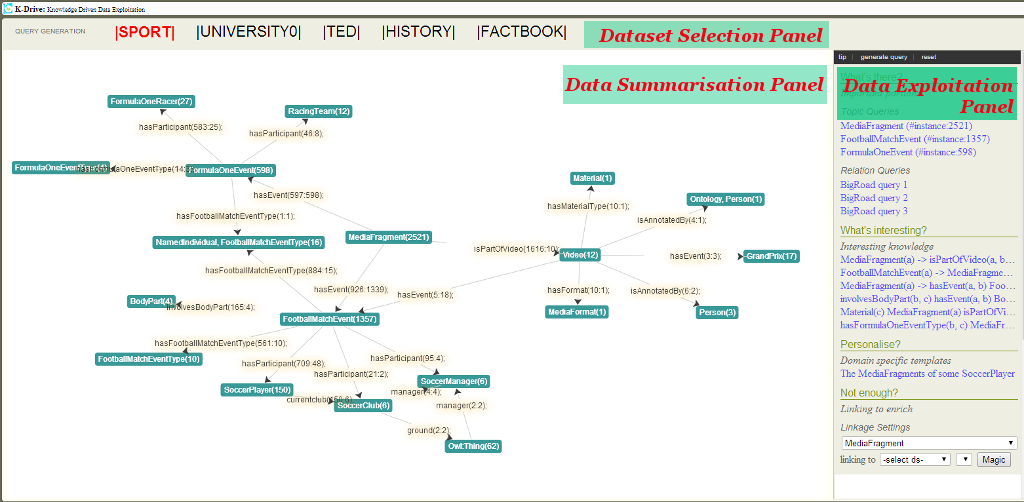
\includegraphics[scale=0.30, trim=12mm 1mm 5cm 1cm]{figures/ui_general_annotated.png}
 \caption{Data Exploitation UI}\label{fig:ui}
\endminipage\hfill
\minipage{0.50\textwidth}
  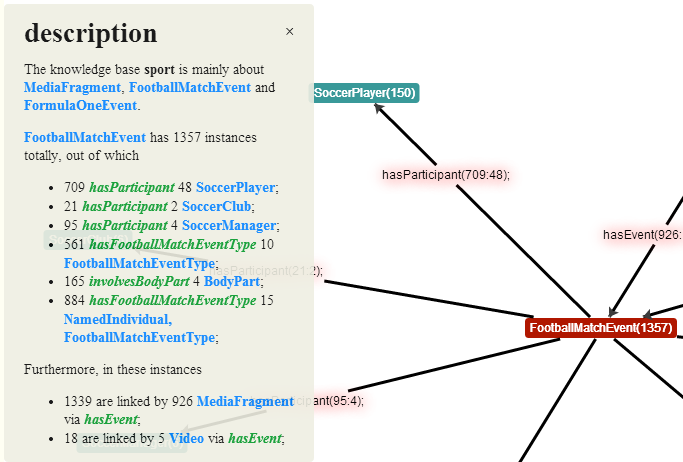
\includegraphics[scale=0.30]{figures/node.png}
  \caption{Node Browsing}\label{fig:node}
\endminipage
\end{figure}
\vspace{-2mm}
To evaluate and demonstrate the effectiveness of the summarisation in data exploitation scenarios, we implemented a summary based data exploitation system for three types of tasks i.e., gaining big picture and browsing, generating queries and enriching datasets. 

The user interface is shown in Figure~\ref{fig:ui} which contains three panels. The upper part is the \emph{Dataset Selection Panel}, which displays the list of datasets in current demo system. To switch to another dataset, one can simply click on its name in this panel. The middle panel is the main interaction and visualisation panel, the \emph{Data Summarisation Panel}. By default, it displays the summarisation of the selected dataset as an interactive graph i.e., the EDP graph. In other situations, relevant subgraphs of the EDP graph will be shown in the data exploitation process. The right panel is the \emph{Data Exploitation Panel}, which shows a bunch of UI components supporting various data exploitation operations.

Given the UI, we now demonstrate a list of data exploitation scenarios to illustrate how the summarisation can help the data exploitation tasks.

\noindent \textbf{The Big Picture and Browsing Operations}
When facing an unfamiliar dataset, users usually pursue a quick and rough \emph{big picture} of it before (s)he can assess whether it is interesting or not, e.g, what are the data describing (concepts), how are the main concepts connected to each other (relations) and which are the important parts (clusters). To help the users gain answers to these questions quickly, as shown in the \emph{Data Summarisation Panel} of Figure~\ref{fig:ui}, the EDP graph is visualised by using force-directed graph drawing techniques~\footnote{Arbor Javascript Library (\url{http://arborjs.org/introduction}) is used for the EDP graph rendering.}. Each node in the graph describes a concept. In addition to the concept name, a node is also attached with the number of instances it has in the dataset. Such statistics(c.f. Figure~\ref{fig:node}) helps to assess the importance of each concept in the dataset (in terms of data portions). The relations between (instances of) these concepts are rendered as edges, and such edges are used to calculate groups of closely related nodes, which are in turn rendered as clusters in the graph.

Two browsing operations are supported on the summary graph. The first is \emph{node browsing}. By clicking on one node in the graph, users can gain detailed description about the concept (c.f. Figure~\ref{fig:node}) including the subgraph centralised on this node which is displayed in the middle panel and the natural language description of the node displayed in a pop-up panel on the left. The second browsing operation is \emph{graph browsing}. After selecting a node, users can keep selecting/de-selecting interconnected nodes in current subgraph to grow or shrink it. This operation enables focused investigation on relations between interested nodes.

\noindent \textbf{Query Generation}
A typical usage on Semantic Web datasets is querying it. Query generation techniques~\cite{pan2013query} are helpful for either novice or advanced users because technical skills and dataset knowledge are prerequisites to write SPARQL queries. Based on the EDP summarisation, we implemented two types of query generation techniques. One is called guided query generation, which generates queries by utilising the EDP graph and statistics information attached in the graph. Such technique is good at generating queries for revealing main concepts and relations in the datasets. These two query types are called \emph{Big City Queries} and \emph{Big Road Queries} in the \emph{Data Exploitation Panel} of the system. They are analogous to big cities and highways in a geography map. The other generation technique makes use of the links in the summarisation to do efficient association rule mining~\cite{pan2013query}. This method is good at revealing insightful knowledge in the data in the form of corresponding graph patterns. Such queries are called \emph{interesting knowledge} in the system. Clicking on any of these generated queries will bring out an illustrating subgraph in the middle part of the UI.  


\noindent \textbf{Dataset Enrichment}
One of the promising features of Semantic Web techniques is the ability to link data silos to form a more valuable information space. Instead of instance-level linkage or ontology mapping, in our system, we introduce a new data linkage operation on EDPs. Such EDP-level linkage makes it possible to investigate what kinds of possibilities would be enabled after cross-dataset EDPs are linked, e.g., previously unanswerable queries might turn to be answerable by linking another dataset via EDP linkage. In the demo, we will demonstrate EDP-linkage between TED and Factbook datasets and show how such linkage can benefit a specific scenario of filtering tenders by country relations.




\section{Demos: The Summary Based Data Exploitations }

\begin{figure}
\minipage{0.40\textwidth}
  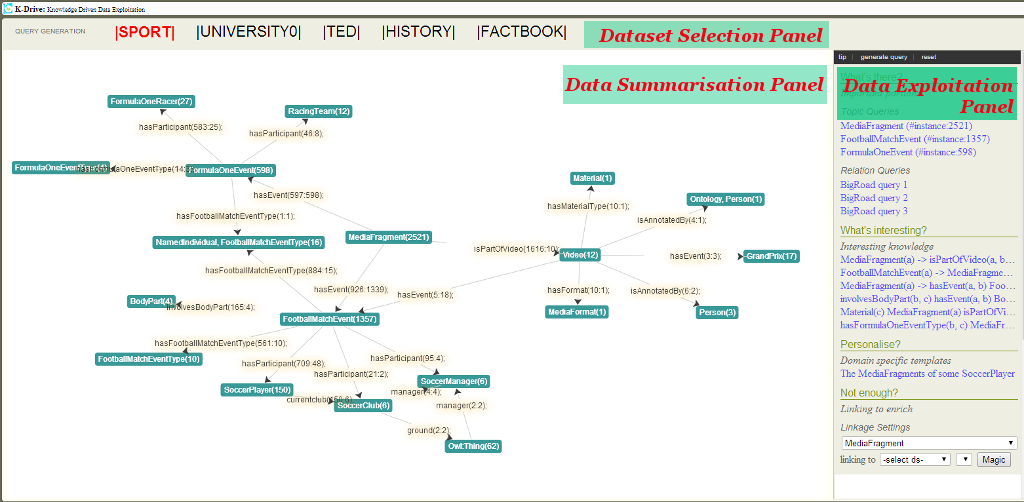
\includegraphics[scale=0.30, trim=12mm 1mm 5cm 1cm]{figures/ui_general_annotated.png}
 \caption{Data Exploitation UI}\label{fig:ui}
\endminipage\hfill
\minipage{0.50\textwidth}
  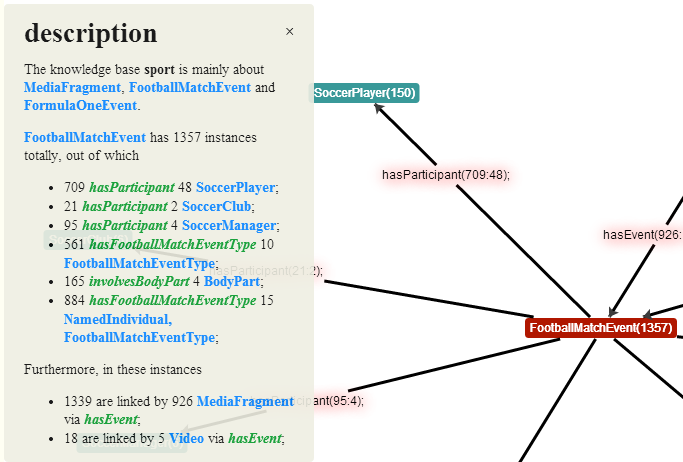
\includegraphics[scale=0.30]{figures/node.png}
  \caption{Node Browsing}\label{fig:node}
\endminipage
\end{figure}
\vspace{-2mm}
To evaluate and demonstrate the effectiveness of the summarisation in data exploitation scenarios, we implemented a summary based data exploitation system for three types of tasks i.e., gaining big picture and browsing, generating queries and enriching datasets. 

The user interface is shown in Figure~\ref{fig:ui} which contains three panels. The upper part is the \emph{Dataset Selection Panel}, which displays the list of datasets in current demo system. To switch to another dataset, one can simply click on its name in this panel. The middle panel is the main interaction and visualisation panel, the \emph{Data Summarisation Panel}. By default, it displays the summarisation of the selected dataset as an interactive graph i.e., the EDP graph. In other situations, relevant subgraphs of the EDP graph will be shown in the data exploitation process. The right panel is the \emph{Data Exploitation Panel}, which shows a bunch of UI components supporting various data exploitation operations.

Given the UI, we now demonstrate a list of data exploitation scenarios to illustrate how the summarisation can help the data exploitation tasks.

\noindent \textbf{The Big Picture and Browsing Operations}
When facing an unfamiliar dataset, users usually pursue a quick and rough \emph{big picture} of it before (s)he can assess whether it is interesting or not, e.g, what are the data describing (concepts), how are the main concepts connected to each other (relations) and which are the important parts (clusters). To help the users gain answers to these questions quickly, as shown in the \emph{Data Summarisation Panel} of Figure~\ref{fig:ui}, the EDP graph is visualised by using force-directed graph drawing techniques~\footnote{Arbor Javascript Library (\url{http://arborjs.org/introduction}) is used for the EDP graph rendering.}. Each node in the graph describes a concept. In addition to the concept name, a node is also attached with the number of instances it has in the dataset. Such statistics(c.f. Figure~\ref{fig:node}) helps to assess the importance of each concept in the dataset (in terms of data portions). The relations between (instances of) these concepts are rendered as edges, and such edges are used to calculate groups of closely related nodes, which are in turn rendered as clusters in the graph.

Two browsing operations are supported on the summary graph. The first is \emph{node browsing}. By clicking on one node in the graph, users can gain detailed description about the concept (c.f. Figure~\ref{fig:node}) including the subgraph centralised on this node which is displayed in the middle panel and the natural language description of the node displayed in a pop-up panel on the left. The second browsing operation is \emph{graph browsing}. After selecting a node, users can keep selecting/de-selecting interconnected nodes in current subgraph to grow or shrink it. This operation enables focused investigation on relations between interested nodes.

\noindent \textbf{Query Generation}
A typical usage on Semantic Web datasets is querying it. Query generation techniques~\cite{pan2013query} are helpful for either novice or advanced users because technical skills and dataset knowledge are prerequisites to write SPARQL queries. Based on the EDP summarisation, we implemented two types of query generation techniques. One is called guided query generation, which generates queries by utilising the EDP graph and statistics information attached in the graph. Such technique is good at generating queries for revealing main concepts and relations in the datasets. These two query types are called \emph{Big City Queries} and \emph{Big Road Queries} in the \emph{Data Exploitation Panel} of the system. They are analogous to big cities and highways in a geography map. The other generation technique makes use of the links in the summarisation to do efficient association rule mining~\cite{pan2013query}. This method is good at revealing insightful knowledge in the data in the form of corresponding graph patterns. Such queries are called \emph{interesting knowledge} in the system. Clicking on any of these generated queries will bring out an illustrating subgraph in the middle part of the UI.  


\noindent \textbf{Dataset Enrichment}
One of the promising features of Semantic Web techniques is the ability to link data silos to form a more valuable information space. Instead of instance-level linkage or ontology mapping, in our system, we introduce a new data linkage operation on EDPs. Such EDP-level linkage makes it possible to investigate what kinds of possibilities would be enabled after cross-dataset EDPs are linked, e.g., previously unanswerable queries might turn to be answerable by linking another dataset via EDP linkage. In the demo, we will demonstrate EDP-linkage between TED and Factbook datasets and show how such linkage can benefit a specific scenario of filtering tenders by country relations.

%\section{Evaluation}\label{sec:Evaluation}
%\subsection{Evaluation settings}

\subsection{Evaluation results}

\subsection{Evaluation discussion}


\section{Conclusions and Future Work}\label{sec:Conclusions}
We described an EDP centralised summarisation, which was shown to be useful for various data exploitation scenarios. The future work will focus on investigating the properties of the summary and in-depth studies in above scenarios.


%*****************************************************************************************************************



% ---- Bibliography ----
%

\bibliography{bibliography}
\bibliographystyle{plain}



\clearpage
\addtocmark[2]{Author Index} % additional numbered TOC entry
\renewcommand{\indexname}{Author Index}
\printindex \clearpage
\addtocmark[2]{Subject Index} % additional numbered TOC entry
\markboth{Subject Index}{Subject Index}
\renewcommand{\indexname}{Subject Index}
%\input{subjidx.ind}
\end{document}
